\section{Goals and Purpose}
A Head-Up display (HUD) is a transparent display that is installed in a number of aircraft today. Located in the pilot’s forward field of view, a HUD presents flight information by using graphical, numerical and symbolical data. This device eliminates the need for pilots to continually transition from head-down instruments to head-up, out-the-window view during critical phases of flight. Currently, a HUD obtains data from an aircraft’s Inertial Measurement Unit (IMU). To display precise and accurate information, the HUD must be carefully aligned to the IRU during installation. However, the current HUD installation process requires specialized equipment and epoxy which is time consuming, costly, and interrupts production line progress for the manufacturer. The goal of this project is to improve the current HUD alignment systems by reducing the installation cost and time required to precisely align flight information to the HUD. Our client, Rockwell Collins, seeks a new alignment methodology that utilizes HUD mounted inertial measurement units.

\section{Current Stage}
At this moment, we have completed most required implementations from the perspectives of both hardware and software sides. Specifically, we have successfully configured the hardware setup for reading two sets of data reading from two separate IMUs, and we have found supported libraries to convert raw data from all three kinds of sensors (accelerometer, gyroscope and magnetometer) to our desired format (quaternions and yaw, pitch, roll) in order to implement the alignment process. Then we also designed and created a simple 3D graphical interface to visualize the real time motion of the the IMUs, and finally, we implemented an algorithm to calibrate and align between the output data from both IMUs. However, we are still on a stage of verifying and testing, we will still have further steps to take for accomplishment.

\section{Remain}
What we left for the project are mostly about the improvement including increasing the accuracy of reading data as well as the UI display, and we are also trying to solve the stretch goal of this project, which is to create the dynamic auto-alignment system algorithm. 

\section{Problems and Solutions}
\begin{itemize}
	\item \textbf{Accuracy of GUI display}
	\\The previous UI display works with showing the object rotation based on the delta angle between the current angle of the IMU with the previous angle of the previous position of the animation object. However, this method would add accumulated error/offset to the UI program since the input IMU data will more or less have error. To solve this problem, we decide to reset the plane object for each frame generated by the algorithm. For each frame we delete the old plane, create a new plane, and rotate it based only on the new angle. In this way, we will not accumulate the error from the previous reading and only focussed on the new reading.\\

	\item \textbf{Visualization problem for 2D GUI}
	\\Our previous GUI have a 2D gauge-like looks to it. It looks more like a car dashboard rather than a real plane HUD. This GUI serve our purpose of showing the data really well. However, it is hard to visualize the change on the plane for each angle. Our team is determined to give the best for this project and decided to improve on our GUI. To solve this problem, we create a new GUI that visualize the change of angle to a plane object. We create this GUI by using a python sublanguage called vpython. We also use the pySerial library to connect the GUI to the Arduino part of the project.\\

	\item \textbf{Statistical Analysis Implementation}
	\\During the previous iteration of the statistical analysis portion of the project I create the algorithm in the Visual studio. However, when we want to change the GUI to vpython, I need to translate all the algorithm to python. A big problem for this is that python doesn't have the statistics library that I use in Visual Studio, which means that I have to write the statistical analysis portion of this project from scratch. Also, putting statistical analysis algorithm in the GUI.py file will also reduce the performance on the GUI, since Python runtime performance is slow. To solve and prevent this problem from happening again, we decide to put the statistical analysis portion of the code in the Arduino. With the help of my teammates, we successfully implemented the statistical analysis algorithm in the Arduino. Other benefits of doing the statistical analysis portion in the Arduino is that we can solve all the calculation in advance and only send the good value to the GUI. In this way, the GUI will receive less data which makes the overhead of the GUI way smaller.\\
\end{itemize}



\section{Sample Code}
For our demonstration system, we use vPython to create the graphical user interface (GUI) of the project. Following is the function that we use to reset the plane for each plane in our GUI. This function takes the plane object, the yaw, pitch, roll angles, and the color of the plane as an input. This function will delete the plane object input and create a new plane with the rotation specified by the yaw, pitch, and roll angles input. We also specified the color so we can know which plane are we reseting. Red color is for the plane from the HUD sensor and the Green color is for the plane from the aircraft sensor.\\

\begin{lstlisting}[language=python]
	def reset(plane, yaw, pitch, roll, color):
		plane.visible = False
		del plane
		#time.sleep(0.05)
		plane = vp.frame()
		vp.ellipsoid(frame=plane, pos=(0,0,0), length=8, height=2.5, width=2.5, color=color, opacity=0.5)
		vp.pyramid(frame=plane, pos=(-1,0,0), size=(4,6,1), color=color, opacity=0.5)
		vp.pyramid(frame=plane, pos=(-3.5,0,1), size=(2,1,2), color=color, opacity=0.5)
		plane.rotate(angle=math.pi/2, axis=(-1,0,0), origin=(0,0,0))
		plane.rotate(angle=roll, axis=(1,0,0))		#pitch
		plane.rotate(angle=yaw, axis=(0,1,0))		#roll
		plane.rotate(angle=-pitch, axis=(0,0,1))	#yaw
\end{lstlisting}

This piece of code is the bone of our GUI. This code performs the animation for the GUI. This code set a while loop that loop over for the animation at a rate of 30 frames per second. This code reads the datas from the serial input, and put it into a specified array. Then from that array, we use those datas as the yaw, pitch, and roll angles for the planes. Next, we call the reset function to update the object for animation. Finally, we set the termination condition for this loop when the serial input is closed.\\

\begin{lstlisting}[language=python]
	while True:
		# performed rate for animation
		vp.rate(30)	
		while SERIRAL_INPUT.inWaiting() == 0:
			pass

		serial_line = SERIRAL_INPUT.readline()
		c = readData(serial_line)
		if len(c) == 6:	# filter out none numeric data input
			print c
			imu1.cur_yaw = float(c[0]) * DtoR
			imu1.cur_pitch = float(c[1]) * DtoR
			imu1.cur_roll = float(c[2]) * DtoR

			imu2.cur_yaw = float(c[3]) * DtoR
			imu2.cur_pitch = float(c[4]) * DtoR
			imu2.cur_roll = float(c[5]) * DtoR

		plane = reset(plane, imu1.cur_yaw, imu1.cur_pitch, imu1.cur_roll, vp.color.red)
		plane2 = reset(plane2, imu2.cur_yaw, imu2.cur_pitch, imu2.cur_roll, vp.color.green)
		text2 = text_reset(text2, imu1.cur_yaw, -4, -9, 0)
		text3 = text_reset(text3, imu1.cur_pitch, 0, -9, 0)
		text4 = text_reset(text4, imu1.cur_roll, 4, -9, 0 )
		text5 = text_reset(text5, imu2.cur_yaw, -4, -10, 0)
		text6 = text_reset(text6, imu2.cur_pitch, 0, -10, 0 )
		text7 = text_reset(text7, imu2.cur_roll, 4, -10, 0 )

	SERIRAL_INPUT.close() # Only executes once the loop exits
\end{lstlisting}

\newpage
\section{Write-up (results)}
Our project required a two part calibration process. First, each IMU was configured to output its individual sensor data. During IMU configuration, an initial calibration was performed to discover each sensors individual bias. Once the biases were known, we removed them from future readings. Next, the alignment offset discovery required a calibration process to produce a result within an acceptable range. We found the offset between two IMUs (airplane and HUD) after taking a number of samples from each device, the difference between each pair of samples and the average of those differences. Multiple data readings were required in each part of calibration to remove inaccuracies.\\

\begin{itemize}
\item \textbf{Statistical Analysis}
\\For our statistical analysis we applied a 95\% confidence interval to our offset data to ensure that the resulting offset was precise. By using a confidence interval we can retrieve a valid offset value as soon as the quaternion value converges. Without using a confidence interval, we could end up with an erroneous value.\\

Our implementation originally stored 60 samples each for the yaw, pitch and roll offset before using those values to find the confidence interval. Unfortunately, the microcontroller's memory is limited, which makes finding a precise value difficult. We were able to increase the number of samples and increase our performance by taking the offsets of each yaw, pitch and roll sequentially, thus tripling our sample sizes.\\

Currently, the confidence interval is only being applied to the offsets between each device. Further improvements may be gained by increased use of statistical analysis. One such improvement would be to apply our analysis during calibration. The current process relies on a simple average of a single stream of data.\\

\item \textbf{Demonstration Result}
\\Unfortunately, at this time our demonstration system does not allow us to make measured adjustments to our sensors in real time. Without real time adjustments, the difference between the pitch value might actually just be a result of opposite axis bias. The following graph presents the pitch value of each sensor over time. The rise in the red line represents the physical motion of a single sensor up by roughly 2 degrees. The decline in the red line represents the physical motion of the same sensor back to its initial location. The figure~\ref{fig:plot} demonstrates the physical change in offset with a measured change in offset.

	\begin{figure}
		\centering
	 		\caption{Offset Plot on Arduino IDE}
	      	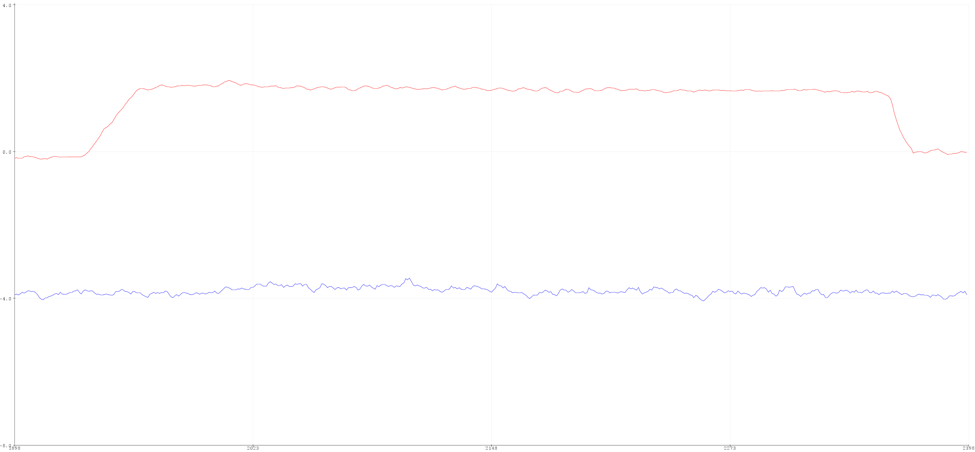
\includegraphics[width=\textwidth,height=\textheight,keepaspectratio]{plot}
	    \label{fig:plot}
	\end{figure}

\end{itemize}

